\documentclass{article}
\usepackage{amsmath,amsthm,amsfonts,amssymb,amscd}
\usepackage{fullpage}
\usepackage{lastpage}
\usepackage{enumerate}
\usepackage{fancyhdr}
\usepackage[percent]{overpic}
\usepackage{mathrsfs}
\usepackage{wrapfig}
\usepackage{multirow}
\usepackage{amsmath}
\usepackage{amssymb}
\usepackage{amscd}
\usepackage{lscape}
\usepackage{graphicx}
\usepackage[usenames,dvipsnames]{color}
\usepackage{listings}
\usepackage[usenames,dvipsnames,svgnames,table]{xcolor}
\usepackage[left=2.5cm,right=2.5cm,top=2.5cm,bottom=2.5cm, headsep = 0.9cm]{geometry}
\usepackage{verbdef}
\setlength{\parindent}{0.0in}
\setlength{\parskip}{0.0in}
\usepackage{setspace}
\definecolor{gray}{RGB}{90,90,90}
\usepackage[colorlinks=true, linktoc=all, linkcolor=blue]{hyperref}

\pagestyle{plain}

\usepackage{Sweave}
\begin{document}
\Sconcordance{concordance:exampledoc.tex:exampledoc.Rnw:%
1 28 1 1 0 8 1 1 4 3 0 3 1 3 0 2 2 4 0 2 2 1 0 1 1 3 0 1 2 4 1 1 2 10 0 %
2 2 68 0 2 2 14 0 2 2 4 0 1 2 1 1 1 2 32 0 1 2 3 1 1 2 5 0 2 2 5 0 1 2 %
8 1}


\centerline{\large{\textbf{Examples of some \texttt{uwIntroStats} Functions}}}
\centerline{\textbf{Author: Brian D. Williamson}}
\tableofcontents
$$$$
\section{Introduction}
This document is meant to illustrate the use of some of the major \texttt{uwIntroStats} functions. The examples will be shown with R code and output. For more options, see the help files provided with the package. Thus, before starting, load both the packages that \texttt{uwIntroStats} relies on:
\begin{Schunk}
\begin{Sinput}
> ## uwIntroStats relies on the Exact, survival, 
> ## plyr, and sandwich packages
> library(Exact)
> library(survival)
> library(plyr)
> library(sandwich)
\end{Sinput}
\end{Schunk}
Now load the \texttt{uwIntroStats} package (if you don't have it installed, go to ``emersonstatistics.com/R'' and download the appropriate file).
\begin{Schunk}
\begin{Sinput}
> library(uwIntroStats)
\end{Sinput}
\end{Schunk}
We will also be working with the \texttt{mri} dataset, so prepare that as well:
\begin{Schunk}
\begin{Sinput}
> data(mri)
> attach(mri)
\end{Sinput}
\end{Schunk}
The reference manual for the \texttt{mri} dataset can be found on ``emersonstatistics.com/Datasets''. 

\section{Descriptive Statistics}
\subsection{\texttt{descrip()}}
Now that we have our package and dataset loaded, we can delve deeper into the functions. When we first get a dataset, we often want to find some descriptive statistics. The most common are the number of observations a variable has, the number of missing observations, the mean, median, standard deviation, and some others. The default \texttt{descrip()} function will give all of this and more to us. Let's say we wanted to get descriptive statistics for \texttt{age}:
\begin{Schunk}
\begin{Sinput}
> descrip(age)
\end{Sinput}
\begin{Soutput}
       N     Msng  Mean      Std Dev    Min       25%        Mdn       75%     
age:     735     0   74.57     5.451     65.00    71.000000   74.00     78.00  
        Max     
age:     99.00  
\end{Soutput}
\end{Schunk}
However, what if we are interested in the whole dataset? We can do this too!
\begin{Schunk}
\begin{Sinput}
> descrip(mri)
\end{Sinput}
\begin{Soutput}
            N     Msng  Mean      Std Dev    Min       25%          Mdn     
    ptid:     735     0   368.0     212.3     1.000   1.845000e+02   368.0  
 mridate:     735     0   76423     31896     10192   6.664200e+04   80992  
     age:     735     0   74.57     5.451     65.00   7.100000e+01   74.00  
    male:     735     0   0.4980    0.5003    0.0000  0.000000e+00   0.0000 
    race:     735     0   1.318     0.6659    1.000   1.000000e+00   1.000  
  weight:     735     0   159.9     30.74     74.00   1.385000e+02   158.0  
  height:     735     0   165.8     9.710     139.0   1.580000e+02   165.9  
 packyrs:     735     1   19.60     27.11     0.0000  0.000000e+00   6.500  
 yrsquit:     735     0   9.661     14.10     0.0000  0.000000e+00   0.0000 
   alcoh:     735     0   2.109     4.852     0.0000  0.000000e+00  0.01920 
 physact:     735     0   1.922     2.052     0.0000  5.537500e-01   1.312  
     chf:     735     0  0.05578    0.2297    0.0000  0.000000e+00   0.0000 
     chd:     735     0   0.3347    0.6862    0.0000  0.000000e+00   0.0000 
  stroke:     735     0   0.2367    0.6207    0.0000  0.000000e+00   0.0000 
diabetes:     735     0   0.1075    0.3099    0.0000  0.000000e+00   0.0000 
 genhlth:     735     0   2.588     0.9382    1.000   2.000000e+00   3.000  
     ldl:     735    10   125.8     33.60     11.00   1.020000e+02   125.0  
     alb:     735     2   3.994     0.2690    3.200   3.800000e+00   4.000  
     crt:     735     2   1.064     0.3030    0.5000  9.000000e-01   1.000  
     plt:     735     7   246.0     65.80     92.00   2.017500e+02   239.0  
     sbp:     735     0   131.1     19.66     78.00   1.180000e+02   130.0  
     aai:     735     9   1.103     0.1828    0.3171  1.026900e+00   1.112  
     fev:     735    10   2.207     0.6875    0.4083  1.745000e+00   2.158  
    dsst:     735    12   41.06     12.71     0.0000  3.200000e+01   40.00  
 atrophy:     735     0   35.98     12.92     5.000   2.700000e+01   35.00  
   whgrd:     735     1   2.007     1.410     0.0000  1.000000e+00   2.000  
  numinf:     735     0   0.6109    0.9895    0.0000  0.000000e+00   0.0000 
  volinf:     735     1   3.223     17.36     0.0000  0.000000e+00   0.0000 
 obstime:     735     0    1804     392.3     68.00   1.837000e+03    1879  
   death:     735     0   0.1810    0.3852    0.0000  0.000000e+00   0.0000 
             75%       Max      
    ptid:     551.5      735.0  
 mridate:     91392    1.232e+05
     age:     78.00      99.00  
    male:     1.000      1.000  
    race:     1.000      4.000  
  weight:     179.0      264.0  
  height:     173.2      190.5  
 packyrs:     33.75      240.0  
 yrsquit:     18.50      56.00  
   alcoh:     1.144      35.00  
 physact:     2.513      13.81  
     chf:     0.0000     1.000  
     chd:     0.0000     2.000  
  stroke:     0.0000     2.000  
diabetes:     0.0000     1.000  
 genhlth:     3.000      5.000  
     ldl:     147.0      247.0  
     alb:     4.200      5.000  
     crt:     1.200      4.000  
     plt:     285.0      539.0  
     sbp:     142.0      210.0  
     aai:     1.207      1.728  
     fev:     2.649      4.471  
    dsst:     50.00      82.00  
 atrophy:     44.00      84.00  
   whgrd:     3.000      9.000  
  numinf:     1.000      5.000  
  volinf:    0.09420     197.0  
 obstime:      2044      2159   
   death:     0.0000     1.000  
\end{Soutput}
\end{Schunk}
Now we know that the \texttt{male} variable can stratify the data. A natural question to ask is: what are the descriptive statistics for age stratified by sex?
\begin{Schunk}
\begin{Sinput}
> descrip(age, strata=male)
\end{Sinput}
\begin{Soutput}
               N     Msng  Mean      Std Dev    Min       25%        Mdn     
age:  All        735     0   74.57     5.451     65.00    71.000000   74.00  
age:    Str  0   369     0   74.41     5.258     65.00    71.000000   73.00  
age:    Str  1   366     0   74.73     5.642     66.00    71.000000   74.00  
                75%       Max     
age:  All        78.00     99.00  
age:    Str  0   78.00     91.00  
age:    Str  1   78.00     99.00  
\end{Soutput}
\end{Schunk}
Other functionality of \texttt{descrip()}, as with all of the functions in R, can be found by typing
\begin{Schunk}
\begin{Sinput}
> ?descrip
\end{Sinput}
\end{Schunk}
\subsection{\texttt{tableStat()}}
The next step is to build tables of descriptive statistics. For example, suppose we wish to have a table with count, row percentage, column percentage, standard deviation, and range. This is easy with \texttt{tableStat()}! We will build this table using \texttt{stroke} as our variable, stratified by \texttt{race} and \texttt{male}
\begin{Schunk}
\begin{Sinput}
> tableStat(stroke, race, male, stat="count=@count@; row%=@row%@ col%=@col%@; sd=@sd@; range = @min@ - @max@")
\end{Sinput}
\begin{Soutput}
Tabled descriptive statistics by strata
Call:
      tableStat.default(variable = stroke, race, male, stat = "count=@count@; row%=@row%@ col%=@col%@; sd=@sd@; range = @min@ - @max@") 
            - NaN denotes strata with no observations
            - NA arises from missing or censored data

Format:  count=Cnt; row%=% of row col%=% of col; sd=SD; range = Min - Max 

         male.0                                                              
race.1   count=286.0; row%= 50.0% col%= 77.5%; sd=0.5184; range = 0.0 - 2.000
race.2   count= 53.0; row%= 51.0% col%= 14.4%; sd=0.4666; range = 0.0 - 2.000
race.3   count= 26.0; row%= 55.3% col%=  7.0%; sd=0.6794; range = 0.0 - 2.000
race.4   count=  4.0; row%= 33.3% col%=  1.1%; sd=0.0000; range = 0.0 - 0.000
race.ALL count=369.0; row%= 50.2% col%=100.0%; sd=0.5219; range = 0.0 - 2.000
         male.1                                                              
race.1   count=286.0; row%= 50.0% col%= 78.1%; sd=0.7032; range = 0.0 - 2.000
race.2   count= 51.0; row%= 49.0% col%= 13.9%; sd=0.7013; range = 0.0 - 2.000
race.3   count= 21.0; row%= 44.7% col%=  5.7%; sd=0.7171; range = 0.0 - 2.000
race.4   count=  8.0; row%= 66.7% col%=  2.2%; sd=0.7071; range = 0.0 - 2.000
race.ALL count=366.0; row%= 49.8% col%=100.0%; sd=0.7010; range = 0.0 - 2.000
         male.ALL                                                            
race.1   count=572.0; row%=100.0% col%= 77.8%; sd=0.6210; range = 0.0 - 2.000
race.2   count=104.0; row%=100.0% col%= 14.1%; sd=0.5974; range = 0.0 - 2.000
race.3   count= 47.0; row%=100.0% col%=  6.4%; sd=0.6889; range = 0.0 - 2.000
race.4   count= 12.0; row%=100.0% col%=  1.6%; sd=0.5774; range = 0.0 - 2.000
race.ALL count=735.0; row%=100.0% col%=100.0%; sd=0.6207; range = 0.0 - 2.000
\end{Soutput}
\end{Schunk}

\section{Plots}
\subsection{Box plots}
As we cover in our document ``An Introduction to R'', box plots can be controversial as a descriptive plot of the data. However, we aimed to mitigate some of those concerns with our box plot function. It is straightforward to add jittered data to the plot (allowing us to see all of the data allows us to see where ``outliers'' really are) and overlay the sample mean and standard deviation - giving us a much better picture of the data. Let's create a boxplot of fev by race:
\begin{Schunk}
\begin{Sinput}
> bplot(fev, race, xlab="Race", ylab="FEV")
\end{Sinput}
\end{Schunk}
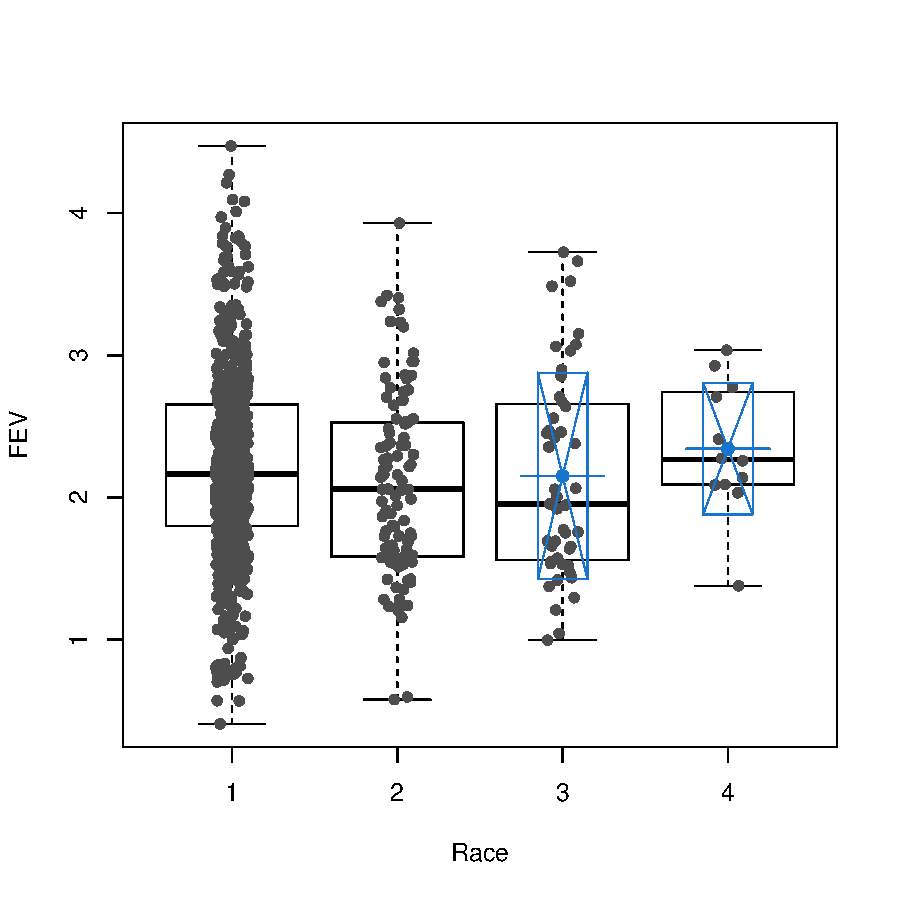
\includegraphics{exampledoc-009}
\\Notice that by default the jittered data is added to the plot, and the plots are overlaid with sample mean and standard deviation. Now we can also stratify by sex:
\begin{Schunk}
\begin{Sinput}
> bplot(fev, race, strata=male, xlab="Race by Sex", ylab="FEV")
\end{Sinput}
\end{Schunk}
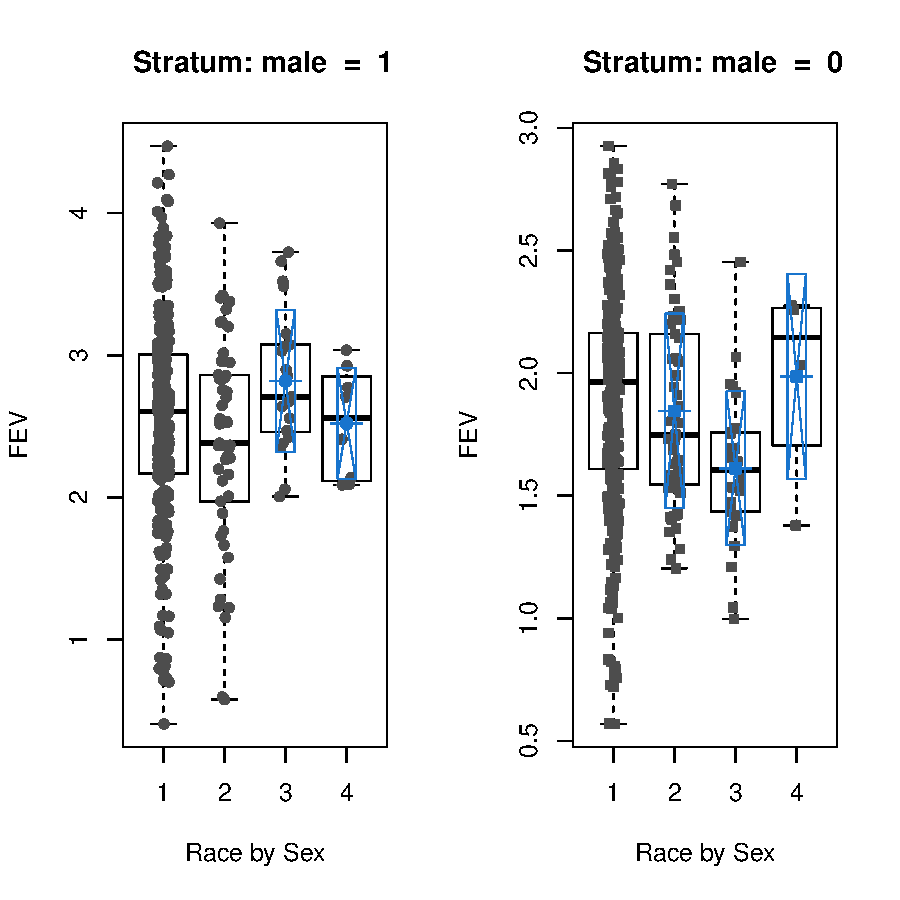
\includegraphics{exampledoc-010}

\subsection{Scatter plots}
We also often wish to view a scatter plot of the data. 

\section{Inference}
\subsection{\texttt{tabulate()}}


\end{document}
